% Q16: 按固定候选 PDF 第1页（印刷页282）的示意图重绘；曲线仅表达向上开口与零点。
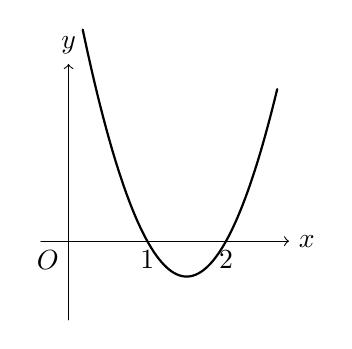
\begin{tikzpicture}[line cap=round,line join=round,scale=1.0]
  \draw[->] (-0.35,0)--(2.8,0) node[right] {$x$};
  \draw[->] (0,-1.0)--(0,2.25) node[above] {$y$};
  \draw[thick,domain=0.18:2.65,samples=80]
    plot (\x,{1.8*(\x-1)*(\x-2)});
  \node[below left] at (0,0) {$O$};
  \node[below] at (1,0) {$1$};
  \node[below] at (2,0) {$2$};
\end{tikzpicture}
